    La interfaz gráfica de la aplicación está desarrollada empleando Java Swing, orientada a un uso intuitivo por parte de los usuarios finales.
    La aplicación permitirá el acceso a los servicios de alquiler de bicicletas a través de una serie de pantallas conectadas por un flujo lógico y sencillo.
    Por falta de tiempo, sólo se ha realizado el diseño de las pantallas relativas al usuario, dejando de lado las pantallas de administración y mantenimiento de estaciones y bicicletas.
    Esta sección será actualizada en futuras versiones del documento para incluir las pantallas restantes.

    \subsection{Resumen de las Pantallas}\label{subsec:resumen-de-las-pantallas}

    A continuación se detallan las principales pantallas de la aplicación:

    \subsubsection{Pantalla 1: Iniciar sesión}
    \begin{itemize}
        \item \textbf{Nombre:} DiaLogin
        \item \textbf{Objetivo:} Permitir al usuario autenticarse en el sistema.
        \item \textbf{Componentes:}
        \begin{itemize}
            \item Campo de texto para correo electrónico.
            \item Campo de texto para contraseña.
            \item Botón ``Iniciar sesión''.
            \item Enlace para registrarse si no se tiene cuenta.
        \end{itemize}
        \item \textbf{Flujo:} Al iniciar sesión con éxito, se redirige a la pantalla principal.
    \end{itemize}

    \subsubsection{Pantalla 2: Principal del usuario}
    \begin{itemize}
        \item \textbf{Nombre:} VPrincipalUsuario
        \item \textbf{Objetivo:} Servir como punto central de acceso a las funciones principales.
        \item \textbf{Componentes:}
        \begin{itemize}
            \item Vista de mapa con la localización de las estaciones.
            \item Botones para ver estaciones, alquilar, devolver bicicleta.
            \item Acceso al perfil del usuario.
        \end{itemize}
        \item \textbf{Flujo:} Permite navegar hacia la selección de estación o a la edición del perfil.
    \end{itemize}

    \subsubsection{Pantalla 3: Bicicletas en una estación}
    \begin{itemize}
        \item \textbf{Nombre:} DiaBicis
        \item \textbf{Objetivo:} Mostrar bicicletas disponibles en una estación concreta.
        \item \textbf{Componentes:}
        \begin{itemize}
            \item Lista de bicicletas con identificador, tipo y estado.
            \item Botón de reserva/alquiler.
        \end{itemize}
    \end{itemize}

    \subsubsection{Pantalla 4: Perfil de usuario}
    \begin{itemize}
        \item \textbf{Nombre:} DiaUsuario
        \item \textbf{Objetivo:} Permitir la visualización y edición de los datos personales.
        \item \textbf{Componentes:}
        \begin{itemize}
            \item Nombre, correo electrónico, idioma preferido.
            \item Historial de alquileres.
            \item Botón ``Editar perfil''.
        \end{itemize}
    \end{itemize}

    \subsubsection{Pantalla 5: Selección de idioma}
    \begin{itemize}
        \item \textbf{Nombre:} VIdioma
        \item \textbf{Objetivo:} Configurar el idioma de la aplicación.
        \item \textbf{Componentes:}
        \begin{itemize}
            \item Lista desplegable de idiomas.
            \item Botón ``Guardar''.
        \end{itemize}
    \end{itemize}

    \subsection{Estilo visual y usabilidad}

    La interfaz presenta un diseño sencillo, funcional y adaptado a usuarios con diferentes niveles de experiencia tecnológica. Los colores son neutros y consistentes, y los componentes están dispuestos de manera que facilitan la navegación. Los textos son breves y claros, y los botones tienen etiquetas intuitivas.

    \subsection{Diagrama de navegación}\label{subsec:diagrama-de-navegacion}
    El diagrama de navegación muestra cómo se conectan las diferentes pantallas de la aplicación y cómo los usuarios pueden navegar entre ellas. Cada pantalla está conectada a las demás según el flujo lógico del uso de la aplicación, permitiendo un acceso fácil a todas las funcionalidades.
    \begin{figure}[h!]
        \centering
        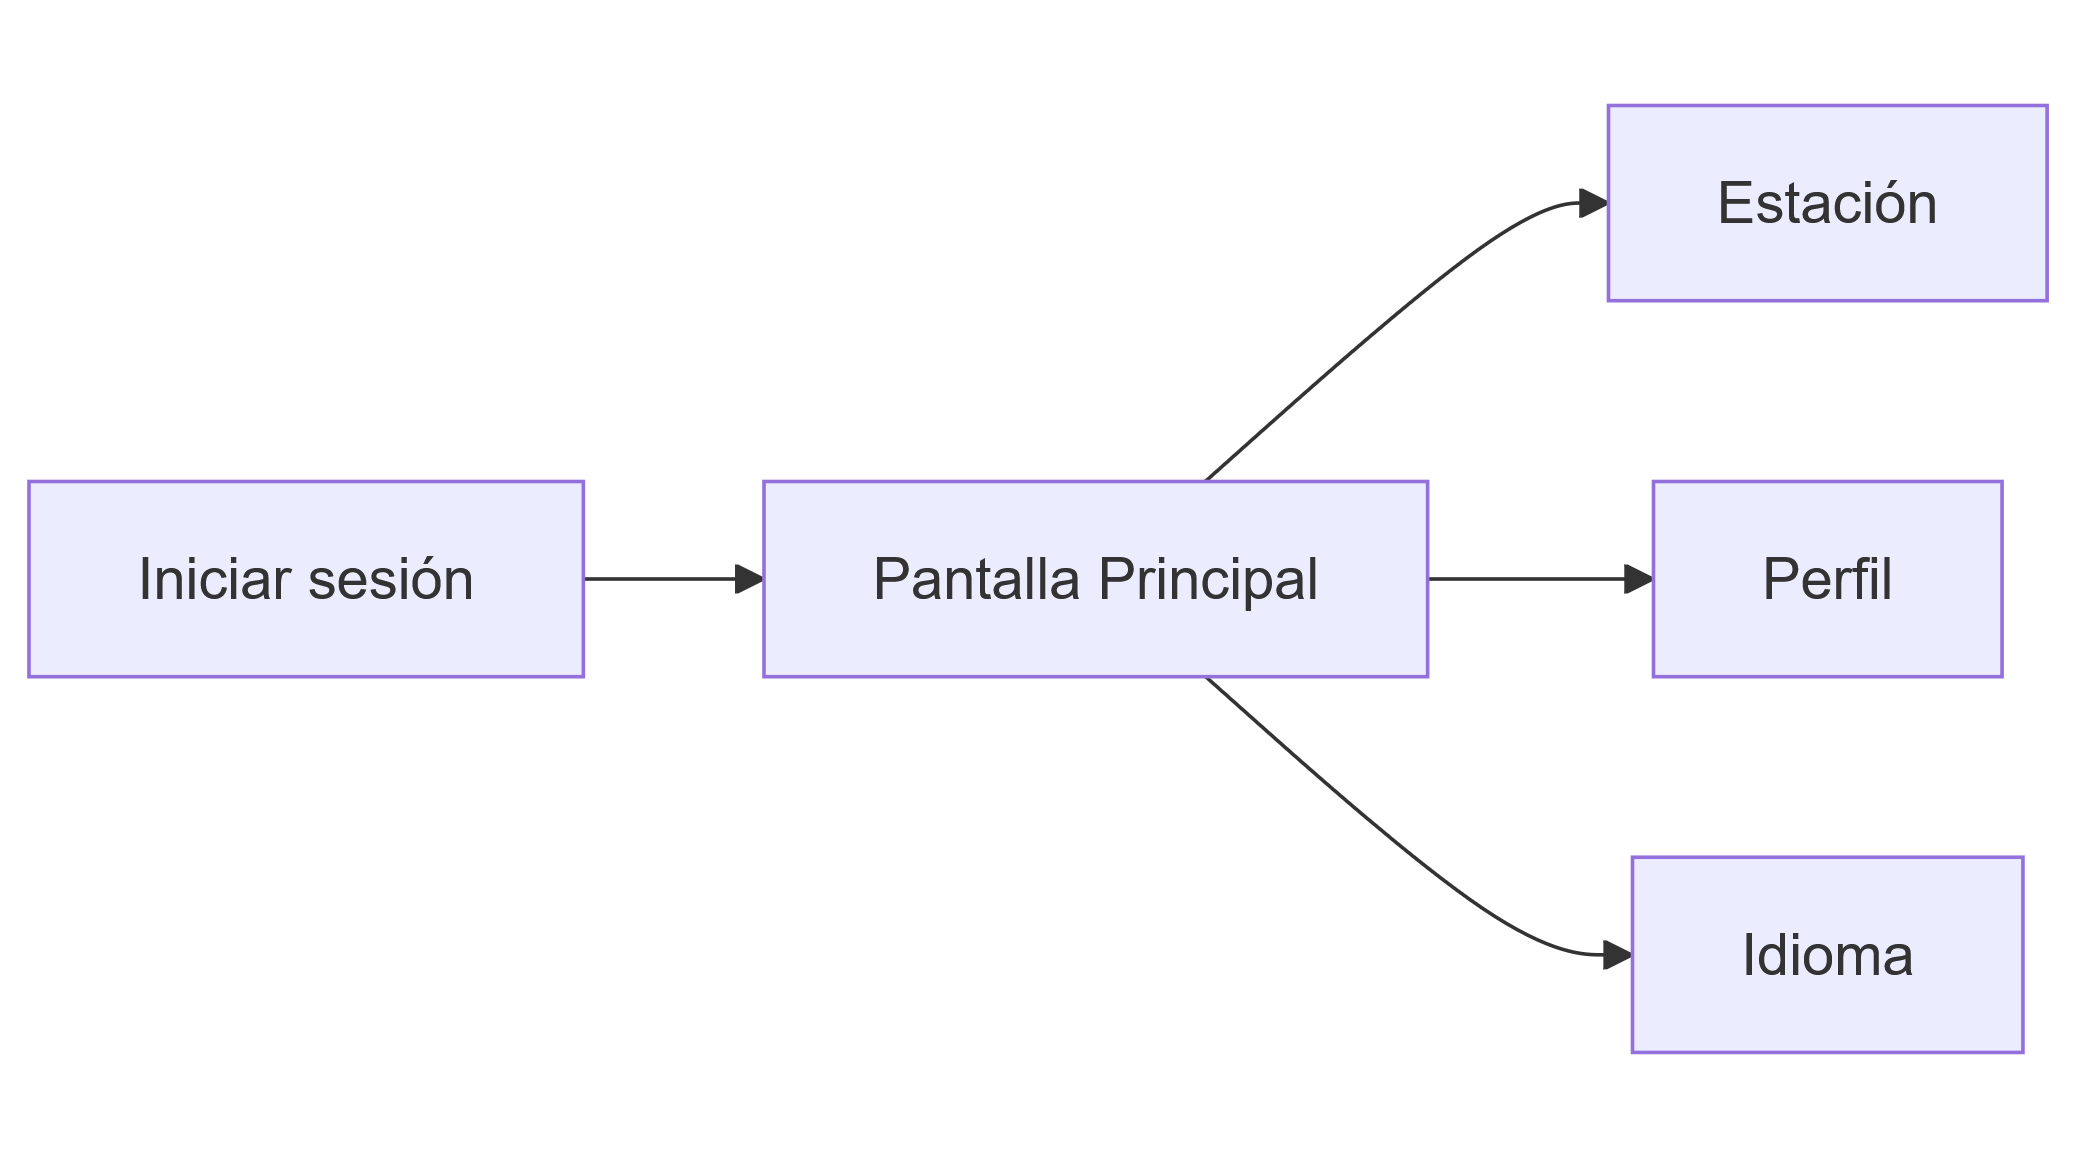
\includegraphics[width=0.7\textwidth]{imagenes/diagrama_navegacion.png}
        \caption{Diagrama de navegación de la aplicación}
        \label{fig:diagrama_navegacion}
    \end{figure}

    \clearpage

    \subsection{Bocetos}\label{subsec:mockups}

    A continuación se presentan los mockups de las pantallas principales de la aplicación.
    Estos mockups ilustran el diseño visual y la disposición de los elementos en cada pantalla.
    Estas han sido creadas con la herramienta Draw.io y se encuentran en formato PNG para su inclusión en el documento. %todo: cita aquí
    \begin{figure}[ht]
        \centering
        \includegraphics{imagenes/bicifast - p1 - Iniciar sesión.drawio}
        \caption{Pantalla 1 - Iniciar sesión}
        \label{fig:bicifast---p1---iniciar-sesion.drawio}
    \end{figure}

    \begin{figure}
        \centering
        \includegraphics[scale=0.50]{imagenes/bicifast - pantalla 2 -principal usuario}
        \caption{Pantalla 2 - Principal del usuario}
        \label{fig:bicifast---pantalla-2--principal-usuario}
    \end{figure}

    \begin{figure}
        \centering
        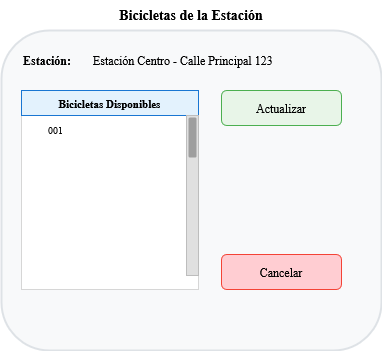
\includegraphics{imagenes/bicifast - pantalla 3 -bicicletas en una estacion.drawio}
        \caption{Pantalla 3 - Bicicletas en una estación}
        \label{fig:bicifast---pantalla-3--bicicletas-en-una-estacion.drawio}
    \end{figure}

    \begin{figure}
        \centering
        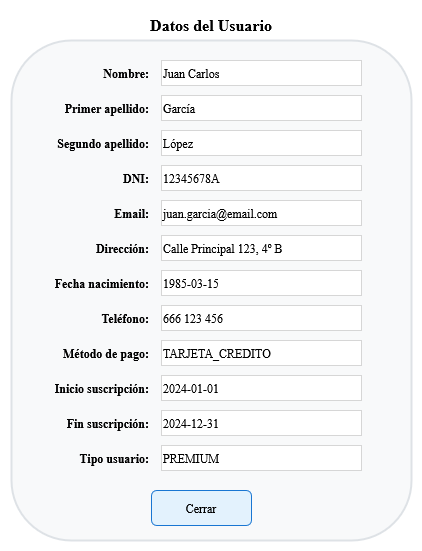
\includegraphics{imagenes/bicifast - pantalla 4 -datos del usuario.drawio}
        \caption{Pantalla 4 - Datos del usuario}
        \label{fig:bicifast---pantalla-4--datos-del-usuario.drawio}
    \end{figure}

    \begin{figure}
        \centering
        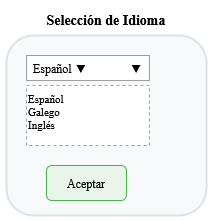
\includegraphics{imagenes/bicifast - pantalla 5 -Seleccion de idiomadrawio}
        \caption{Pantalla 5 - Selección de idioma}
        \label{fig:bicifast---pantalla-5--seleccion-de-idiomadrawio}
    \end{figure}
%    \begin{figure}[H]
%        \centering
%        \includegraphics[width=0.6\textwidth]{ruta/a/bicifast - p1 - Iniciar sesión.drawio.png}
%        \caption{Pantalla 1 - Iniciar sesión}
%    \end{figure}
%
%    \begin{figure}[H]
%        \centering
%        \includegraphics[width=0.6\textwidth]{ruta/a/bicifast - pantalla 2 -principal usuario.png}
%        \caption{Pantalla 2 - Principal del usuario}
%    \end{figure}